\chapter{Little downside and substantial gains result from farming of \textit{Totoaba Macdonaldi}}

\begin{center}
\begin{minipage}{0.9\textwidth}
\singlespacing
This is article is under review at \textit{NPJ Ocean Sustainability} and is joint work with Julia M. Lawson (co-first author), Andrew Steinkruger, Miguel Castellanos-Rico, Garett M. Goto, Miguel A. Cisneros-Mata, Erendira Aceves Bueno, Matthew M. Warham, Adam M. Sachs and Steven D. Gaines\\\\
\end{minipage}

\textbf{Abstract}\par
    \vspace*{.2cm}
    \noindent
    \begin{minipage}{0.9\textwidth}
Illegal wildlife trade poses a growing threat to species globally. Where bans or policy instruments have failed, conservation farming has been considered, which aims to reduce illegal poaching by “flooding the market” with farmed product. However, predicting if farming will succeed necessitates a holistic understanding of how supply and demand interact and how markets will respond. Poaching and illegal trade for totoaba (Totoaba macdonaldi), currently dominated by a Mexican monopolist cartel, has continued unabated despite half a century of prohibitions on international trade and domestic fishing. We investigate if farming can reduce poaching and support a healthy wild population by extending a flexible bioeconomic model of a three-stage illegal supply chain: poachers sell to traders (i.e., middlemen or cartels) who sell to end-markets. While we show under the monopolist a large stable wild population is maintained, this outcome is sensitive to cost parameters. Introducing farming decreases poaching by 29\% or increases poaching by 6\%, and results are robust to changes in cost parameters. Our results upend previous assertions that certain strategic responses will undermine conservation efforts and always result in population collapse. Furthermore, our quantitative framework can be adapted to evaluate conservation farming for other species and market structures.\\\\
Keywords : 
\end{minipage}
\end{center}
    \vfill


\newpage

\section{Introduction}
\onehalfspacing
Illegal wildlife trade is a multi-billion dollar industry that drives biodiversity loss through unsustainable harvest \citep{t_sas-rolfes_illegal_2019}, spreads zoonotic disease \citep{bell_animal_2004}, and threatens animal welfare\citep{baker_rough_2013}. The Convention on International Trade in Endangered Species of Wild Fauna and Flora (CITES) provides a regulatory framework that aims to ensure that international trade of wild animals and plants does not threaten their survival. Yet, for many species, regulatory interventions such as trade bans and controls have failed, and illegal trade in black markets continues to flourish \citep{challender_poaching_2014, challender_towards_2015}. In such instances, supply-side interventions such as conservation farming can theoretically bolster conservation by “flooding the market” with farmed products, leading to reduced market prices and lower poaching incentives \citep{gentry_looking_2019, phelps_framework_2014, tensen_under_2016}. Supply-side interventions have occasionally succeeded at reducing poaching and recovering wild populations – e.g., vicuña and spotted cat \citep{iucn_world_2000, sahley_biological_2007} – but they have also failed – e.g., green python, African elephant \citep{lyons_wildlife_2011, hsiang_does_2016}. Uncertainty around conservation outcomes from market-based approaches has led to continued reliance on trade bans and controls that are often ineffective at reducing poaching.
\\
Determining whether farming will succeed or fail requires a holistic understanding of a specific illegal wildlife market1, including the interplay between market conditions and ecological criteria \citep{challender_understanding_2015}. Studies have pointed to a common set of farming pitfalls. Species with slow individual growth rates and low fecundity are often unable to grow supply quickly enough to displace illegal products. Further, if poaching is very inexpensive, it is impossible for farming to undercut prices 6,8 – e.g., dried seahorses are ‘free’ to poach when retained as bycatch \citep{lawson_low_2017}. Demand-side concerns are focused on substitutability between farmed and wild products. Consumers of wildlife for medicinal or conspicuous purposes often prefer wild products for greater perceived potency or associated social status \citep{dutton_stated_2011, gratwicke_attitudes_2008, fabinyi_historical_2012}. Here, we develop a quantitative framework that comprehensively considers all these pitfalls while accounting for detailed species-specific and market information. 
\\
Another critical factor in driving the success or failure of farming is market structure: illegal markets are often characterized by imperfect competition – where an individual trader or a small number of traders (i.e., middlemen, cartels, gangs, or other criminal organizations) dominate illegal trade and exert significant control over market prices. A bioeconomic model that predicts how imperfectly competitive markets will respond to competition from farming was developed almost two decades ago \citep{bulte_economic_2005, damania_economics_2007}. Predicted strategic responses depend on how a trader chooses to compete with farming. If a trader responds by price setting (an aggressive response where the trader tries to undercut farmed prices and take market shares), then poaching pressure will increase and can lead to the collapse of the wild population. On the other hand, if traders respond by quantity adjustment (a mutually beneficial response where the trader competes on the amount of output produced, letting market prices adjust), poaching pressure is reduced and wild populations have the possibility to increase. This model has been widely used to both justify \citep{biggs_legal_2013,abbott_can_2011} and discourage \citep{tensen_under_2016} prospective farming initiatives. The authors of the original bioeconomic model concluded that farming is a perilous coin toss \citep{bulte_economic_2005, damania_economics_2007}. Here, we expand upon this model and reach a different conclusion: that farming can maintain large, stable wild population sizes that are robust to changes in cost structure under both types of competition. Furthermore, quantity adjustment yields substantial decreases in poaching and is the more likely response because prices and profits are higher than under price setting \citep{singh_price_1984}.
\\
We explore the biological and economic performance of conservation farming for totoaba swim bladder in the context of illegal poaching and trade under different market conditions \citep{froehlich_conservation_2017}. Specifically, we examine the evolution of poaching and wild totoaba biomass, as well as prices and profits for different economic actors. The lifecycle for totoaba has been successfully closed in aquaculture, and the species is currently farmed in Mexico for domestic meat production. Totoaba is endemic to Mexico’s Gulf of California and is threatened by a lucrative illegal international trade for its large swim bladder \citep{c4ads_hooked_2017, environmental_investigation_agency_citess_2019, environmental_investigation_agency_collateral_2016} . A single totoaba swim bladder can sell for up to \$80,000 USD per kilogram in Chinese end markets, where it is purchased for special occasions, gifting, and speculative investment \citep{elephant_action_league_operation_2018, sadovy_de_mitcheson_emerging_2019, martinez_mexican_2021}. For nearly half a century international trade for totoaba has been prohibited, and the legal totoaba commercial fishery has been closed. However, illegal fishing and trade continue and are controlled primarily by a single criminal organization (a cartel) that will likely respond strategically to farming \citep{damania_economics_2007,felbab_brown_organized_2022}  

\begin{figure}[H]
    \centering
    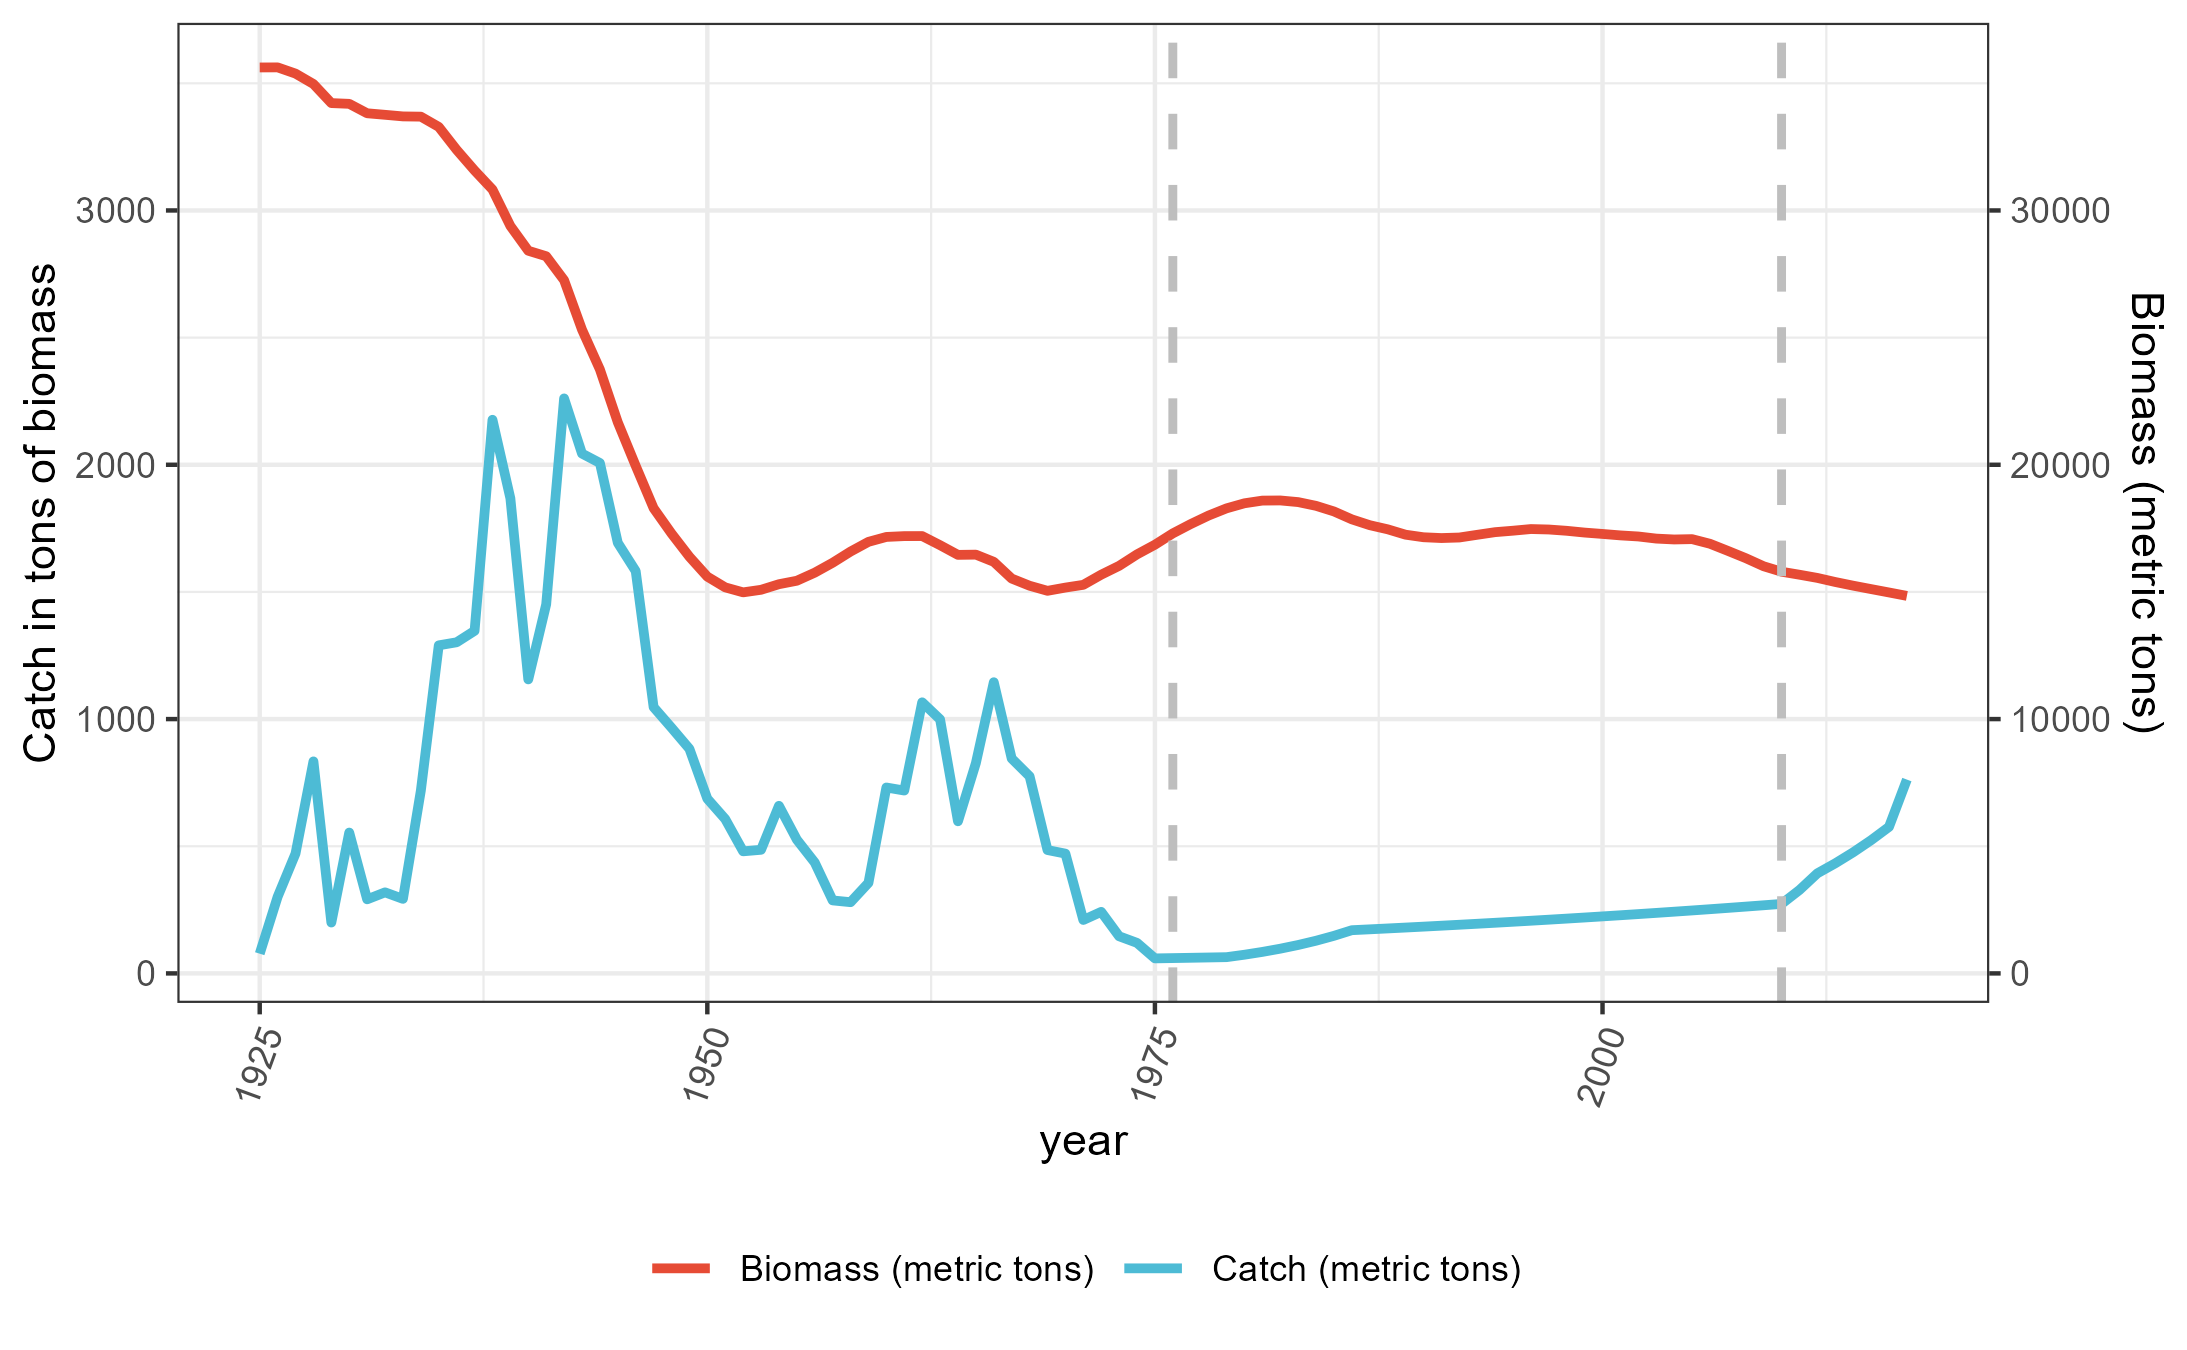
\includegraphics[width=0.8\linewidth]{figures/totoaba/Trends_stock_catch.png}
    \caption{Evolution of totoaba population and catch over time}
    \subcaption*{Dashed lines represent listing as CITES Appendix II species, and cartel takeover, respectively}
    \label{fig:trends_catch}
\end{figure}

There is an urgent need to reduce poaching for totoaba, as the vaquita (Phocoena sinus), a porpoise also endemic to the upper Gulf of California, is caught as bycatch in gillnets used to catch totoaba. The vaquita is on the brink of extinction as there are now fewer than fifteen individuals remaining \citep{rojas-bracho_more_2022}. Furthermore, illegal trade has had negative social welfare consequences, as cartels are increasingly extorting Mexican fishing communities \citep{felbab_brown_organized_2022}. Despite Mexico’s attempts to stop totoaba poaching through various enforcement mechanisms, the country recently received wildlife trade sanctions for taking inadequate action \citep{rojas-bracho_vaquitas_2013,cites_notification_2023}. Conservation farming presents a legal alternative to reduce illegal fishing by manipulating market structure. 
\\
We assemble and leverage a unique wealth of information on the totoaba stock, poaching sector, and farming sector to estimate the effects of market structure on poaching harvest and stock biomass. We focus on the market structure that best characterizes the totoaba trade – a vertical monopoly where a single monopolist trader controls the entire supply chain – and evaluate how this trader will respond strategically to competition from farming. We also show how to identify an effective policy space, where all supply, demand, and market structure parameters align to ensure that conservation farming will reduce poaching. Our results challenge long-standing model conclusions \citep{bulte_economic_2005, damania_economics_2007}, thereby disrupting widely-held beliefs about the impacts of conservation farming. In particular, previous studies cautioned that when a trader responds to farming through price setting, the wild population always declines dramatically. In contrast, we find that for totoaba, price setting can maintain a stable and large population given that as the population size decreases, fishing costs increase. To ensure low retail prices, traders must limit the price they pay to poachers and maintain a viable wild population.

\section{Methods}

We examine the effect of market structure and competition on poaching a population of wild animals using the logistic growth function (Figure \ref{fig:figure2}). The poaching harvest function intersects with population growth producing stable and unstable equilibria. If poaching pressure is high relative to population growth (i.e, when demand is large, or poaching costs are low), a single stable equilibrium point is observed with a low wild abundance (an overharvested population). In the opposite scenario, where poaching pressure is low relative to population growth (i.e, when demand is small, or poaching costs are prohibitive), a single stable equilibrium point is observed with a high wild abundance (a healthy population). Between these extremes, two or three potential equilibria can emerge, with uncertain results that depend on the initial size of the population: a large initial population will result in a high abundance equilibrium point, and a small initial population will result in a low abundance equilibrium point.

\begin{figure}[h]
    \centering
    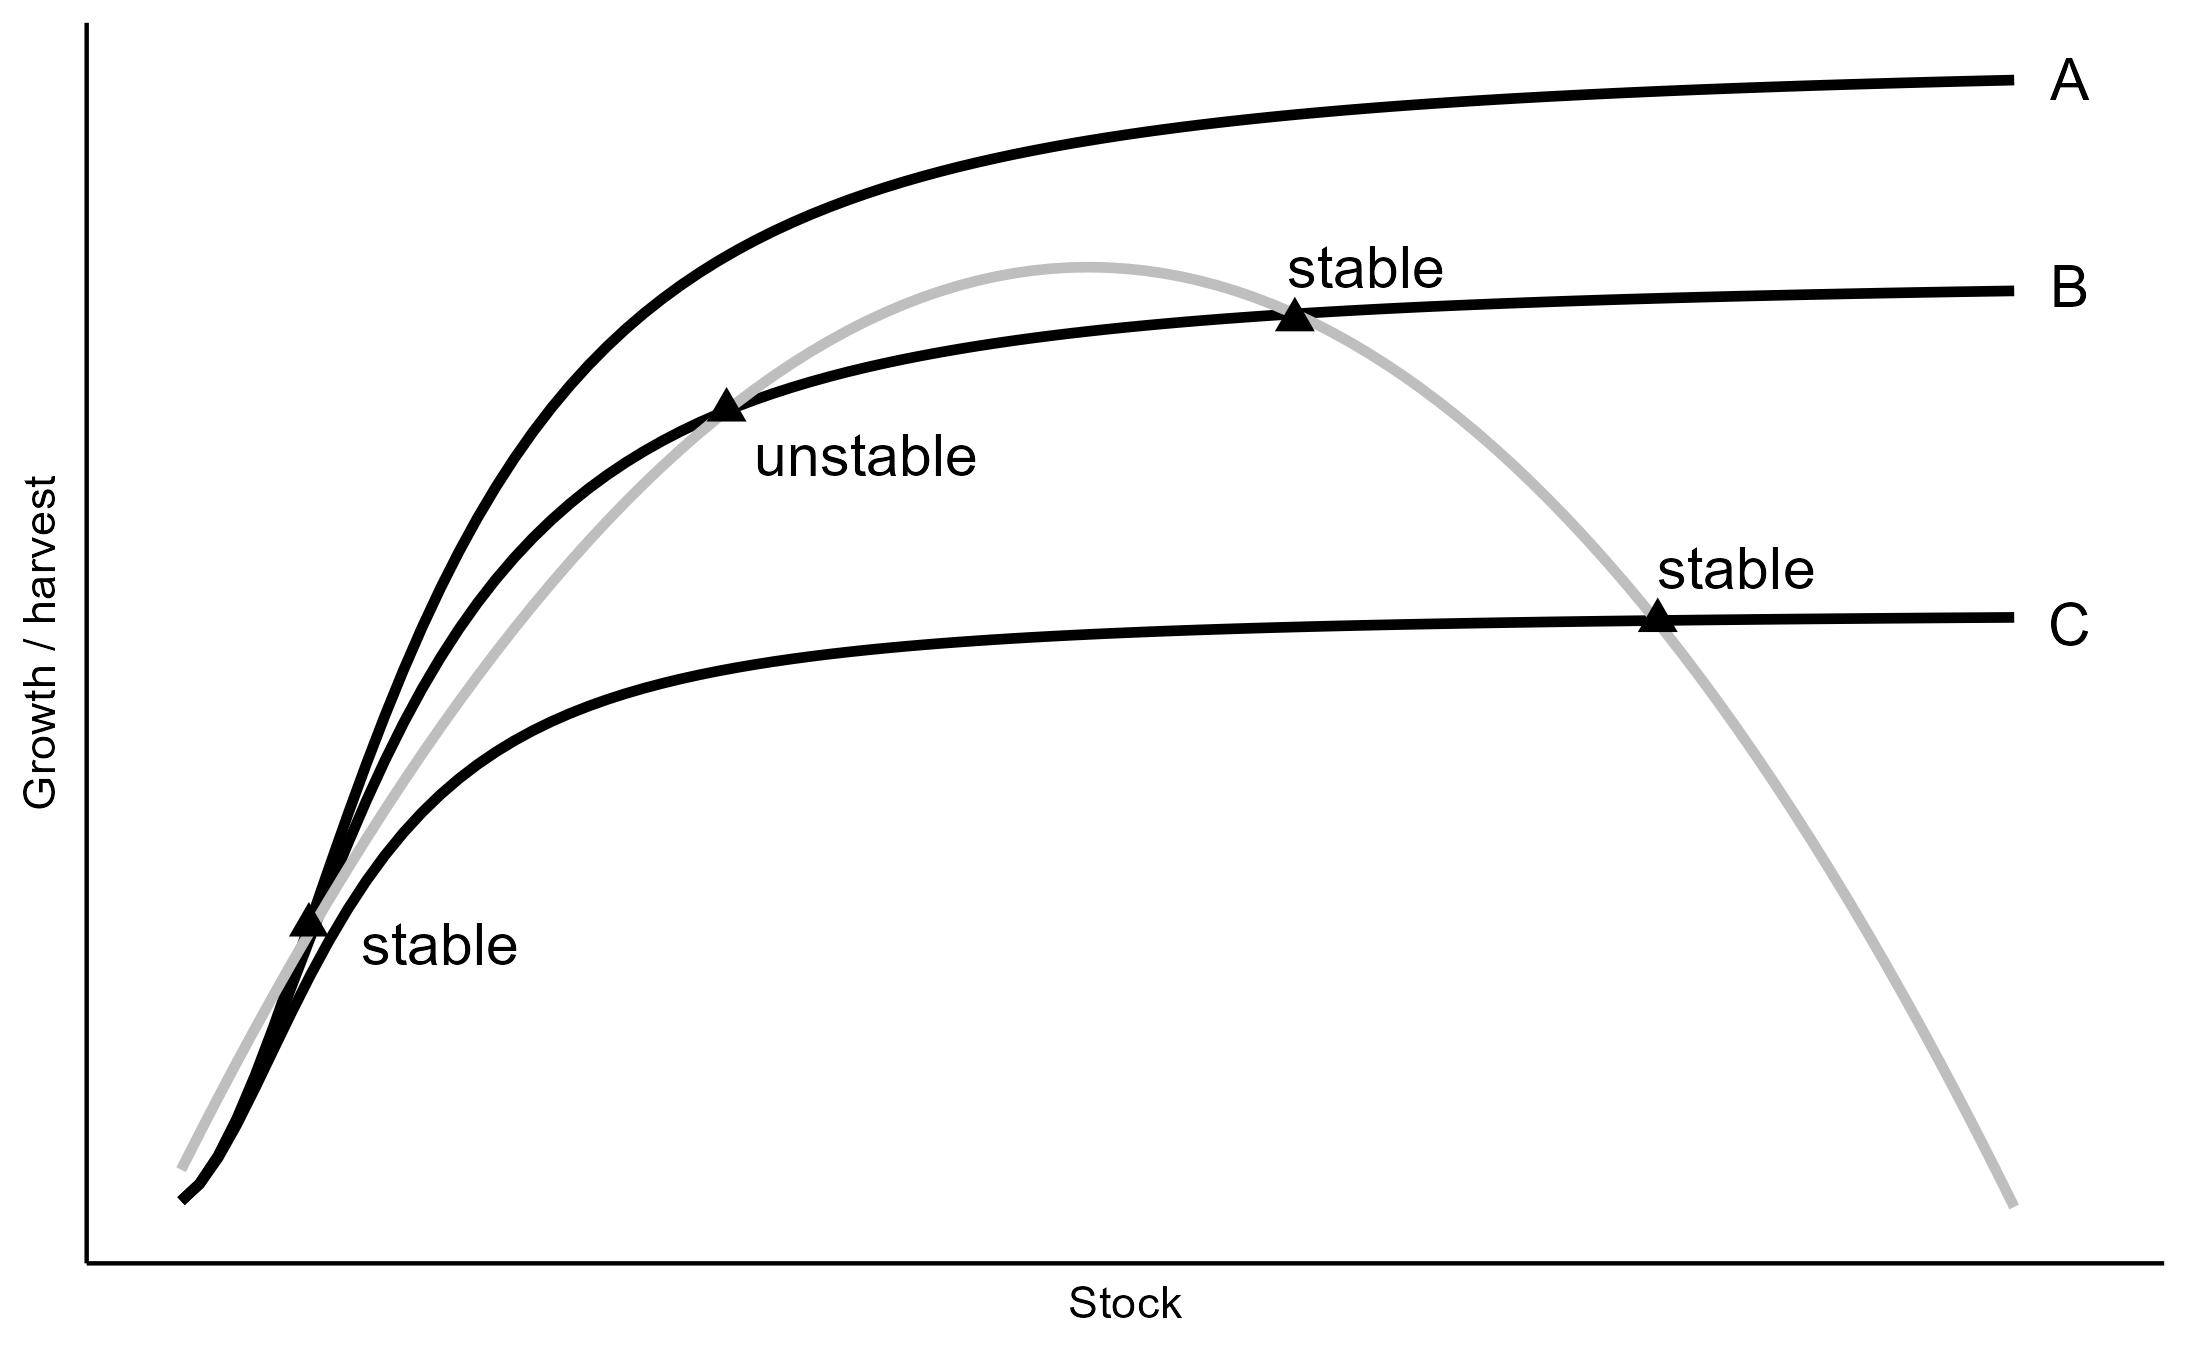
\includegraphics[width=0.85\linewidth]{figures/totoaba/Figure1_potential_equilibria.jpg}
    \caption{Schematic of equilibrium points under different poaching harvest functions}
    \subcaption*{Logistic growth function (light gray) showing equilibria points resulting from three hypothetical poaching harvest functions (black). (A) a single low stable equilibrium point; (B) uncertain outcome, three interior equilibria two of which are stable and one unstable and separating. The long run equilibrium point will depend on the initial size of the population. A large initial population will result in a high abundance equilibrium point, and a small initial population will result in a low abundance equilibrium point; (C) a single high stable equilibrium point.}
    \label{fig:figure2}
\end{figure}

To assess expectations for totoaba, we first calculate equilibrium points for the stock in the absence of conservation farming under vertical monopolistic conditions (hereafter referred to as monopolistic conditions for ease) (Figure \ref{fig:figure3}). A single trader exists in a single location where he is the sole buyer, typical of endemic species such as totoaba \citep{wyatt_differentiating_2020, martinez-alvarado_trafficking_2018}. The trader sells poached harvest on an end market where prices and quantities can be manipulated. 
\\
Next, we add conservation farming to the monopolistic market structure, creating a duopolistic market (Figure \ref{fig:figure3}). We calculate equilibrium points for the totoaba stock if a monopolistic trader responds to conservation farming either in a way that is (a) mutually beneficial by quantity adjustment or (b) aggressive by price setting. From a policy assessment perspective, any scenario where poached harvest produces a single high stable equilibrium point, and the monopolist cartel loses income, presents clear conservation and social welfare benefits.

\begin{figure}[h]
    \centering
    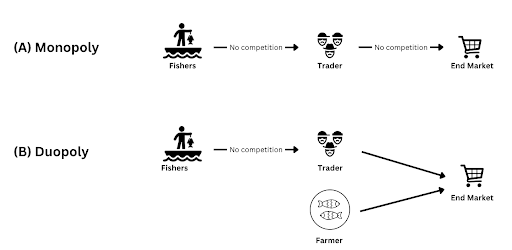
\includegraphics[width=0.85\linewidth]{figures/totoaba/schematic_market.png}
    \caption{Schematic of monopoly and duopoly market structures}
    \subcaption*{(A) monopolistic conditions, where fishers sell to a single trader where they are the sole buyer. This single trader sells poached harvest on an end market where they can manipulate prices and quantities. (B) Next, we add duopoly with farming: A monopolistic trader responds to conservation farming either in a way that is mutually beneficial by quantity adjustment or aggressive by price setting.}
    \label{fig:figure3}
\end{figure}

Here we briefly discuss our methods with an emphasis on the empirical application. Information on our theoretical conclusions from the bioeconomic model we revisited, lemmas and proofs can be found in the Appendix, section \ref{subsection:appendix_toto}. Table \ref{tab:totoaba_functions} summarizes all the functions of the model.  

\subsection{The Poaching Model}

The growth of the fish stock follows a logistic curve and the stock is poached following a Gordon-Schaefer production model. Totoaba population growth parameters were obtained from the 2017 stock assessment, where the carrying capacity ($K$) was $20,226$ mt, and the stock biomass in 2017 was $14,844$ mt \citep{cisneros-mata_evaluacion_2020}. The intrinsic rate of population increase ($r$) was predicted using the \textit{FishLife} package in \textsf{R}, which estimates growth parameters using totoaba-specific life history data from \textit{FishBase} \citep{thorson_predicting_2017}. The growth equation is :
\begin{equation}
g(x) = rx\left(1-\frac{x}{K}\right)
\end{equation}
using a predicted $r$ of $0.20$. We do not consider potential effects of hyperstability of the stock resulting from poaching on seasonal spawning aggregations \citep{erisman_illusion_2011} or age structure.

Poachers optimally determine their effort to maximize their profit, with constant catchability ,$\sigma$, and stock biomass, $x$, obtained from the 2017 stock assessment46, and a linear quadratic cost of effort function, E. The poaching equation is $q =\sigma xE$ where $\sigma =  0.00002. $

Poachers are faced with a linear quadratic cost function $C(E) = W_1 E + W_2E^2$. We calculated two poaching cost parameters $W_1$ (the linear coefficient of the cost function) and $W_2$ (the quadratic coefficient of the cost function) by (a) estimating total and average annual operating costs of the fishing fleet using semi-structured interviews conducted by the authors of this study; and (b) calibrating a linear quadratic cost function that matches historical data and predicts future cost evolution. 

We conducted semi-structured interviews in the upper Gulf of California with two fishing cooperative leaders and four fishers in July and August 2018. These interviews informed annual poaching costs: food and fuel, labor, gear replacement, and bribes paid to fisheries officials. The fishery operates over six months with a variable number of active vessels, monthly fishing days, and sets per day \citep{cisneros-mata_evaluacion_2020}. Poaching costs also include annual fleet-wide costs related to gear confiscations, vessel replacement, and fines, adapted and extrapolated from a summary of law enforcement actions provided by Mexico \citep{noauthor_species_2018}. The cost per fishing trip was estimated to be $\$5,051.26$ during the low season (January and June), $\$8,385.34$ during the mid-season (February and May), and $\$14,386.7$ during the high season (March and April) (supplementary table \ref{tab:costW}). In our analysis we reconstructed a linear quadratic cost function with cumulative effort. We considered effort in each season cumulative with effort in less intense seasons. We used a low-season average cost for effort levels between 0 and low-season effort; for effort levels between low-season effort and cumulated low and mid-season efforts, we used a mid-season average cost.

We estimated the corresponding poaching cost parameters to match the observed average cost and modeled marginal costs at historical levels (resulting in cost parameters $W_1 = 12,200$ \& $W_2 = 0.57$). Our low sample size precludes a robust statistical estimation of these cost parameters, e.g., of the historical cost function and of the evolution of costs if the fishery were to increase. To account for this uncertainty, we run a sensitivity analysis on two dimensions of costs. First, we use different estimates for the average cost and reconstructed total costs, ranging from $-10\%$ to $+30\%$ of our high season average cost estimates. Second, we test weights for the linear and quadratic costs, ranging from a purely linear cost ($W_1 = 14,386,7$, $W_2 = 0$) to a purely quadratic cost ($W_1 = 0$; $W_2 = 3,74$).
 
The resulting poaching profit function is calculated as follows:
\begin{equation}
\Pi = p\sigma x E - W_1E - W_2E^2
\end{equation}

Traders operate on the end market, taking prices as given (competitive scenario) or determining prices (monopolistic scenario) to maximize profits. Traders face a linear demand function. We estimate a linear demand function by regressing price data on estimated catch from 2014 to 201746, yielding the equation $p(q) = \alpha - \beta q$ where the intercept, $\alpha$, is \$1,625,837 USD and the slope coefficient, $\beta$, is \$1,563.75 USD (see supplementary table \ref{tab:demand}). Price data were obtained from available literature that provided estimated weight and value of totoaba maw seizures 24,26,50,51. In addition to the literature review, valuable insights were obtained through personal communication with Wild Aid Investigators (pers. comm. Anonymous Wild Aid Investigators, 2018) as well as with local fishers and cooperative leaders in the upper Gulf of California, as previously described. The information shared by investigators and stakeholders was aggregated with the existing data from the literature. To ensure consistency and comparability, we standardized the weight measurements to grams and the currency values to US dollars. We assume that annual catch reaches the market during the same year, i.e, there is no stockpiling. As data are notoriously difficult to acquire for illegal trade, we pool observations and estimate a stationary demand function (supplementary table \ref{tab:demand}).

Traders buy totoaba from poachers at \textbf{price $s$} (USD/metric ton). The price paid to poachers balances demand from traders and supply to poachers. It decreases as the population increases, as fishing becomes less demanding. Traders also pay a unit transaction cost c (USD/metric ton), which we conservatively estimated to be zero. At a minimum this unit transaction cost includes transport (land and air travel), and payment to two or three ‘runners’ who carry up to ten swim bladders each (pers. comm. Anonymous Wild Aid Investigators, 2018). We know through anecdotal evidence that unit transaction costs $c$ are likely large \citep{elephant_action_league_operation_2018}. However, due to scarce evidence, we used a value of $c=0$ thus adopting a conservative strategy.
\subsection{The Farming Model}
We use a linear profit model for aquaculture and estimate a unit farming production cost parameter $v$ (USD/metric ton) using annual operational costs (labor, feed, vessel fuel, facility and administrative fees), as well as annual maintenance of pens (including cleaning) and vessels, using information provided by existing aquaculture facilities (supplementary table \ref{tab:costv}). Population growth rates differ in the wild and in captivity. Using captive growth rates obtained from personal communication with totoaba aquaculture producers, we consider harvestable size to be between 4.5 and 5 years old (an adult weight of $21.43$ – $27.2$ kg), associated with a swim bladder size between $417$ – $529$ g (supplementary figure \ref{fig:vbgf}). A minimum farmed harvestable size of 4.5 years closely corresponds to the mean swim bladder size (500 g) and estimated adult totoaba size (25.7 kg), as reported in surveys of individuals harvested in the wild \citep{cisneros-mata_evaluacion_2020}. We considered this to be the size at which farmed totoaba would be competitive with the average wild-caught totoaba. We assume that aquaculture operates on a homogenous rotation \citep{faustmann1849, mitra_faustmann_1986}. The implications of this assumption are discussed in the appendix \ref{subsec:aquaculture}. We compute the farming cost per metric ton as the capitalized sum of annual costs over 4.5 years at a $10\%$ interest rate.
\subsection{Demand}
We use a linear demand function in the case of the vertical monopoly, estimated using price and catch data from 2014 to 2017 (see table \ref{tab:demand}), such that $p^w = \alpha^w - \beta^w q^w$. Upon the introduction of aquaculture, following \cite{singh_price_1984} and \cite{damania_economics_2007}, we include a substitutability parameter $\gamma$, which measures the imperfect substitutability between farmed and wild products in the linear demand functions. When farmed products are introduced, the linear demand function is modified such that $p^i(q^i,q^k)=\alpha_i – \beta_i q^i – \gamma q^k$ where $q^i$ and $q^f$ indicate the supply from the wild ($w$) and the farmed supply ($f$). This demand system emerges from a linear quadratic utility function in Supplementary Text (section 1.3.2). When demand intercept $\alpha_i$s are equal, and and own price effect $\beta_i=\beta_j = \gamma$ are equal, products are perfect substitutes. When demand intercepts are equal, but own price effects differ ($\beta_i \neq \beta_j$), then $\frac{\gamma^2}{\beta_i \beta_j}$ denotes the degree of product substitutability. 
At present, there has been no stated preference investigation for wild and farmed totoaba swim bladders in Chinese end-markets, although we know that the end-market economic value for fish maw is determined by taxon, size, and thickness of swim bladder. Investigative work in Mexico reports that it is challenging to distinguish between wild and farmed specimens \citep{elephant_action_league_operation_2018}. Therefore, we assume high substitutability (75\% product substitutability) and check for smaller substitutability values in our sensitivity analysis (Figure \ref{fig:figure6}) (see supplementary table \ref{tab:params}) for a list of parameters).


\section{Results}
\subsection{Totoaba stock under monopoly is sensitive to cost structure}

We revisit and expand upon a bioeconomic model developed nearly two decades ago which differentiates between poachers and traders and develops a three-stage game \citep{bulte_economic_2005, damania_economics_2007}. The totoaba is an endemic species that is illegally traded by a single trader, a monopolist, who dominates the market. This is the market structure that best characterizes the present consolidated totoaba trade \citep{felbab_brown_organized_2022}. In this setting, a single monopolist trader restricts the supply of wildlife products to consumers, leading to increased prices and profits for the monopolist.

\begin{figure}[h]
    \centering
    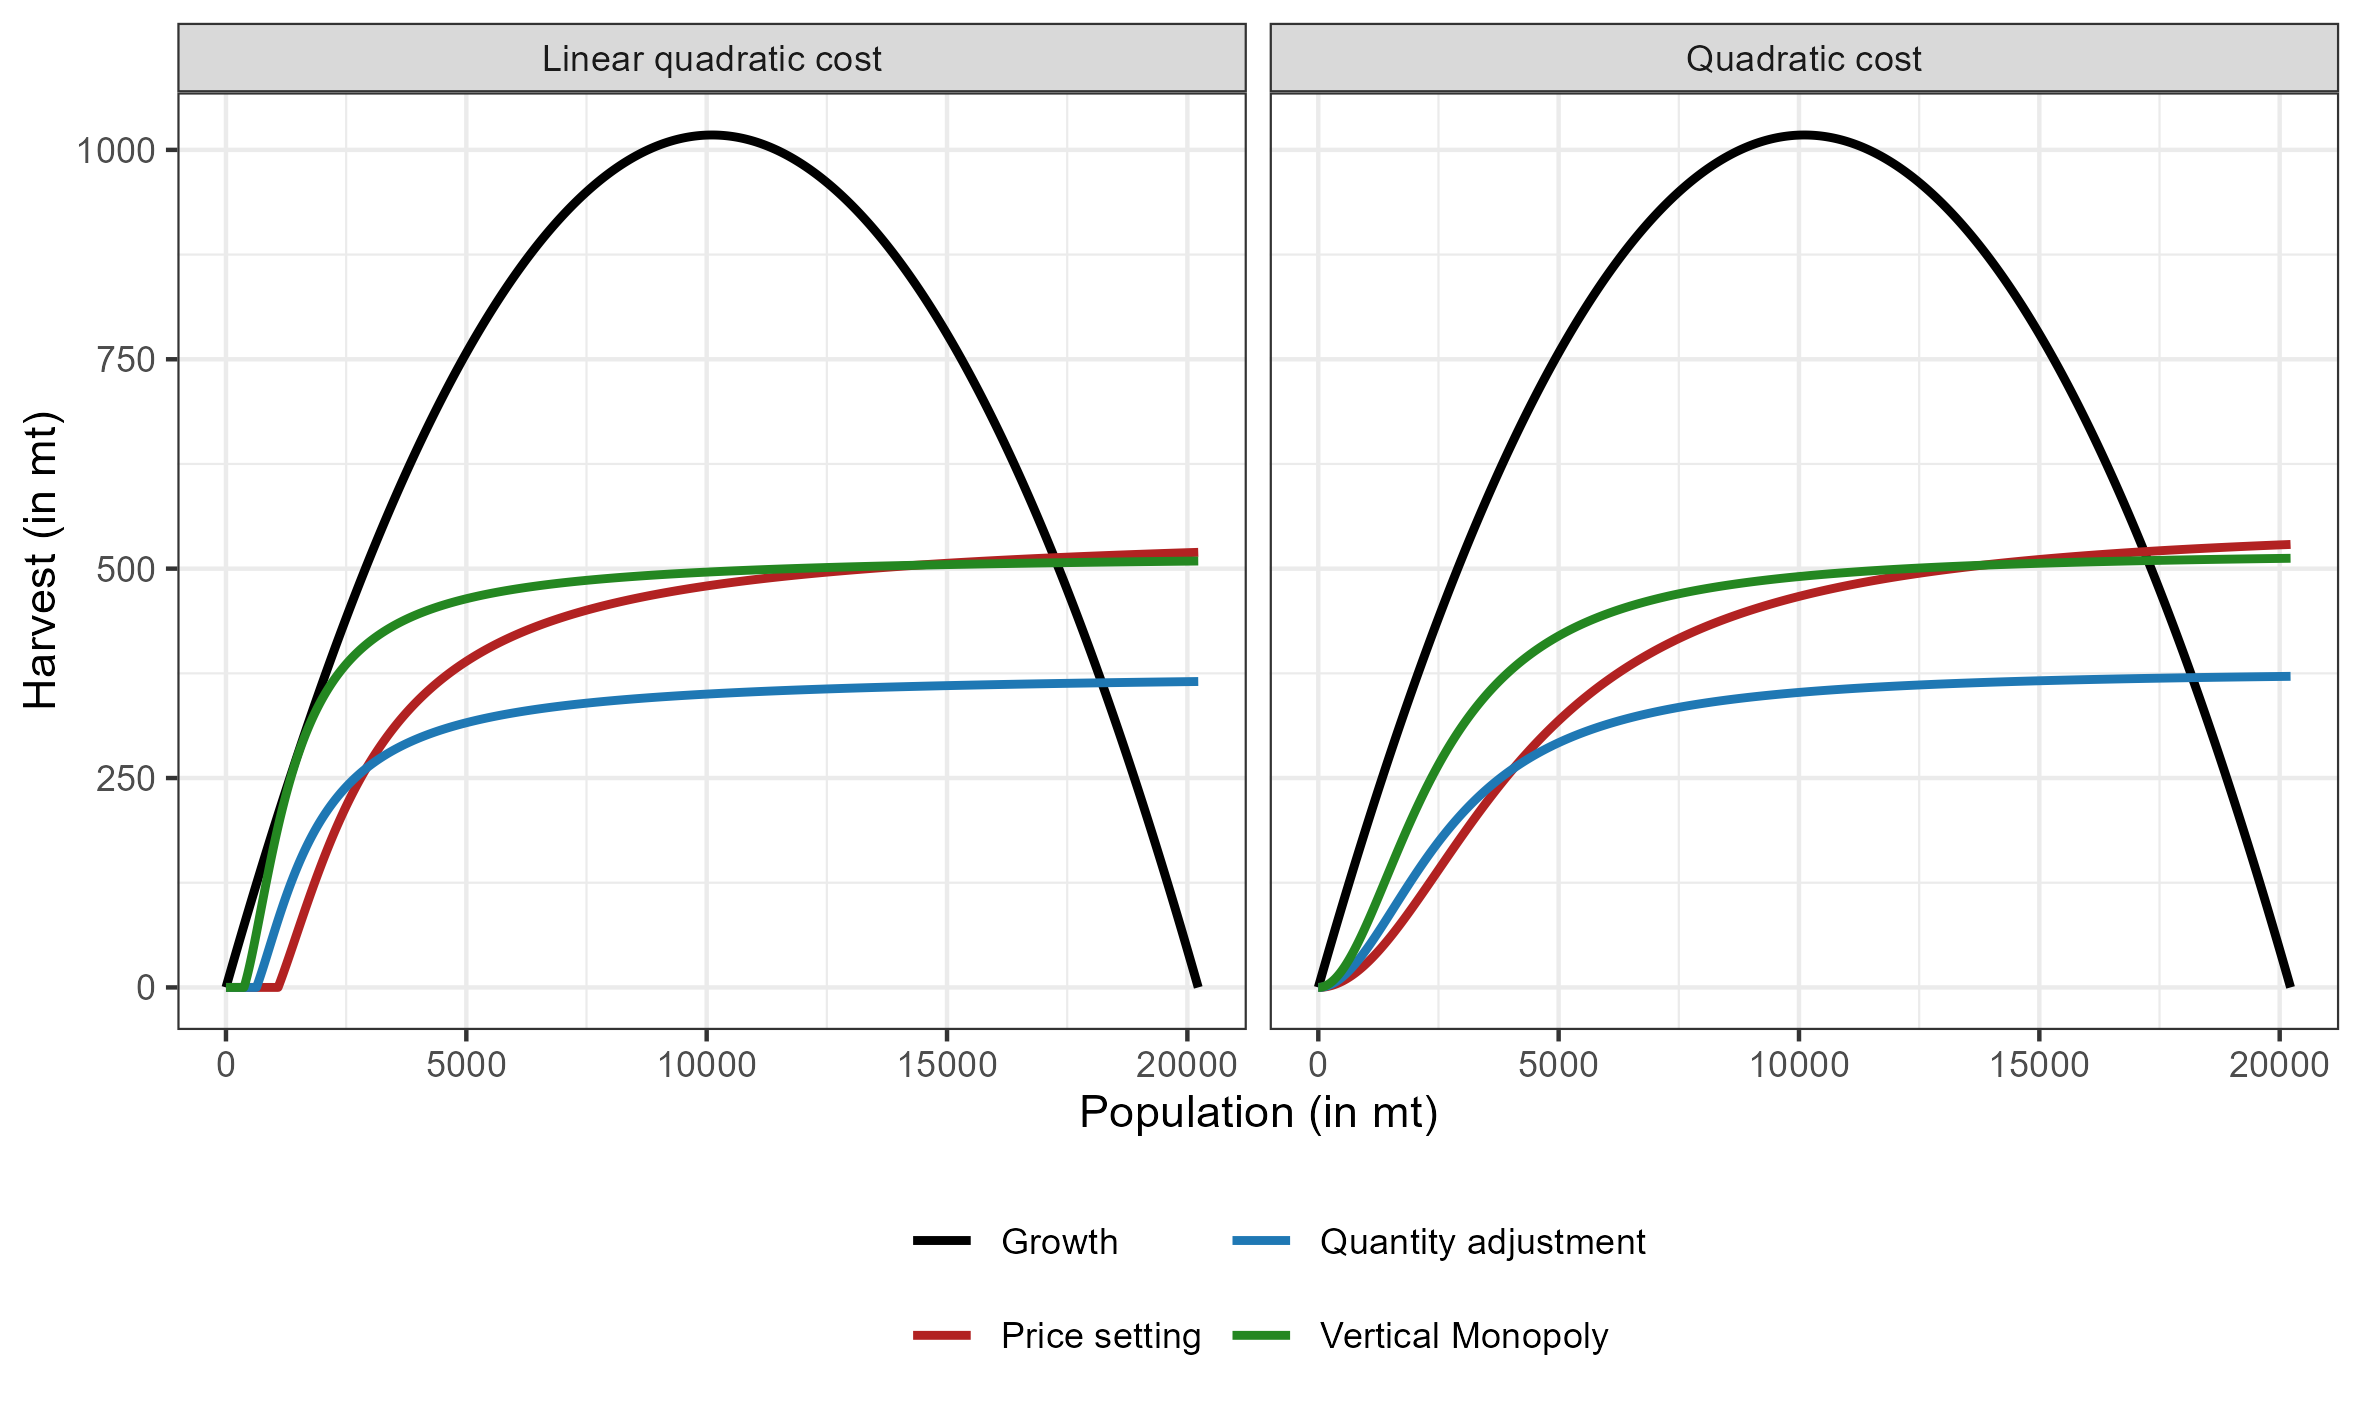
\includegraphics[width=0.85\linewidth]{figures/totoaba/Figure3.png}
    \caption{Equilibrium points for wild totoaba stock under different market structures with (left) a linear quadratic cost structure, and (right) a quadratic cost structure.}
    \subcaption*{Logistic growth function (black) for Totoaba macdonaldi wild stock biomass with intersecting colored lines representing different market structures and competitive responses. Harvest under the status quo vertical monopoly is represented by the green curve. When conservation farming is added to the monopoly scenario the trader can respond either in a mutually beneficial way by adjusting the quantity supplied given a market price (quantity adjustment, in blue). Alternatively, the trader can respond aggressively and try to set a price that undercuts the price of farmed products, resulting in increased poaching (price setting, in red)}
    \label{fig:figure4}
\end{figure}

We initially calculate equilibrium points for totoaba assuming a quadratic cost structure, consistent with the original model, before calculating equilibrium points under a linear quadratic cost structure (Figure \ref{fig:figure4}). Under the quadratic cost structure used in the original bioeconomic model, the totoaba wild stock biomass remains at a high steady-state equilibrium of $17,259$ mt. However, we expand upon the quadratic cost structure, introducing a linear quadratic cost structure to account for energy costs associated with fishing. A linear quadratic cost structure more accurately represents new poachers being recruited to the fishery as fishing opportunities increase \citep{pereau_triple_2012, clark_worldwide_2007}.

We find that under monopoly the linear quadratic cost structure is sensitive to cost parameter specifications, where relatively small changes in cost parameters can cause multiple steady states to emerge (Figure \ref{fig:figure5}). If an increase in poaching comes at a small cost increase compared to historical average costs, the aggregate cost is close to linear (e.g. $W_2 = 0.47$) and below, compared to baseline $W_2 = 0.57$). In this case, a low steady-state equilibrium of $1,106$ mt, an unstable intermediate equilibrium arises at $1,842$ mt and a high stable steady-state equilibrium of $17,277$ mt in the vertical monopoly. Our model uses the best available information on the totoaba fishery, but uncertainty surrounding the projected evolution of fishery-wide poaching costs warrants a cautious assessment of monopoly performances: while it could maintain a healthy population, it can also lead to stock collapse.

\begin{figure}[h]
    \centering
    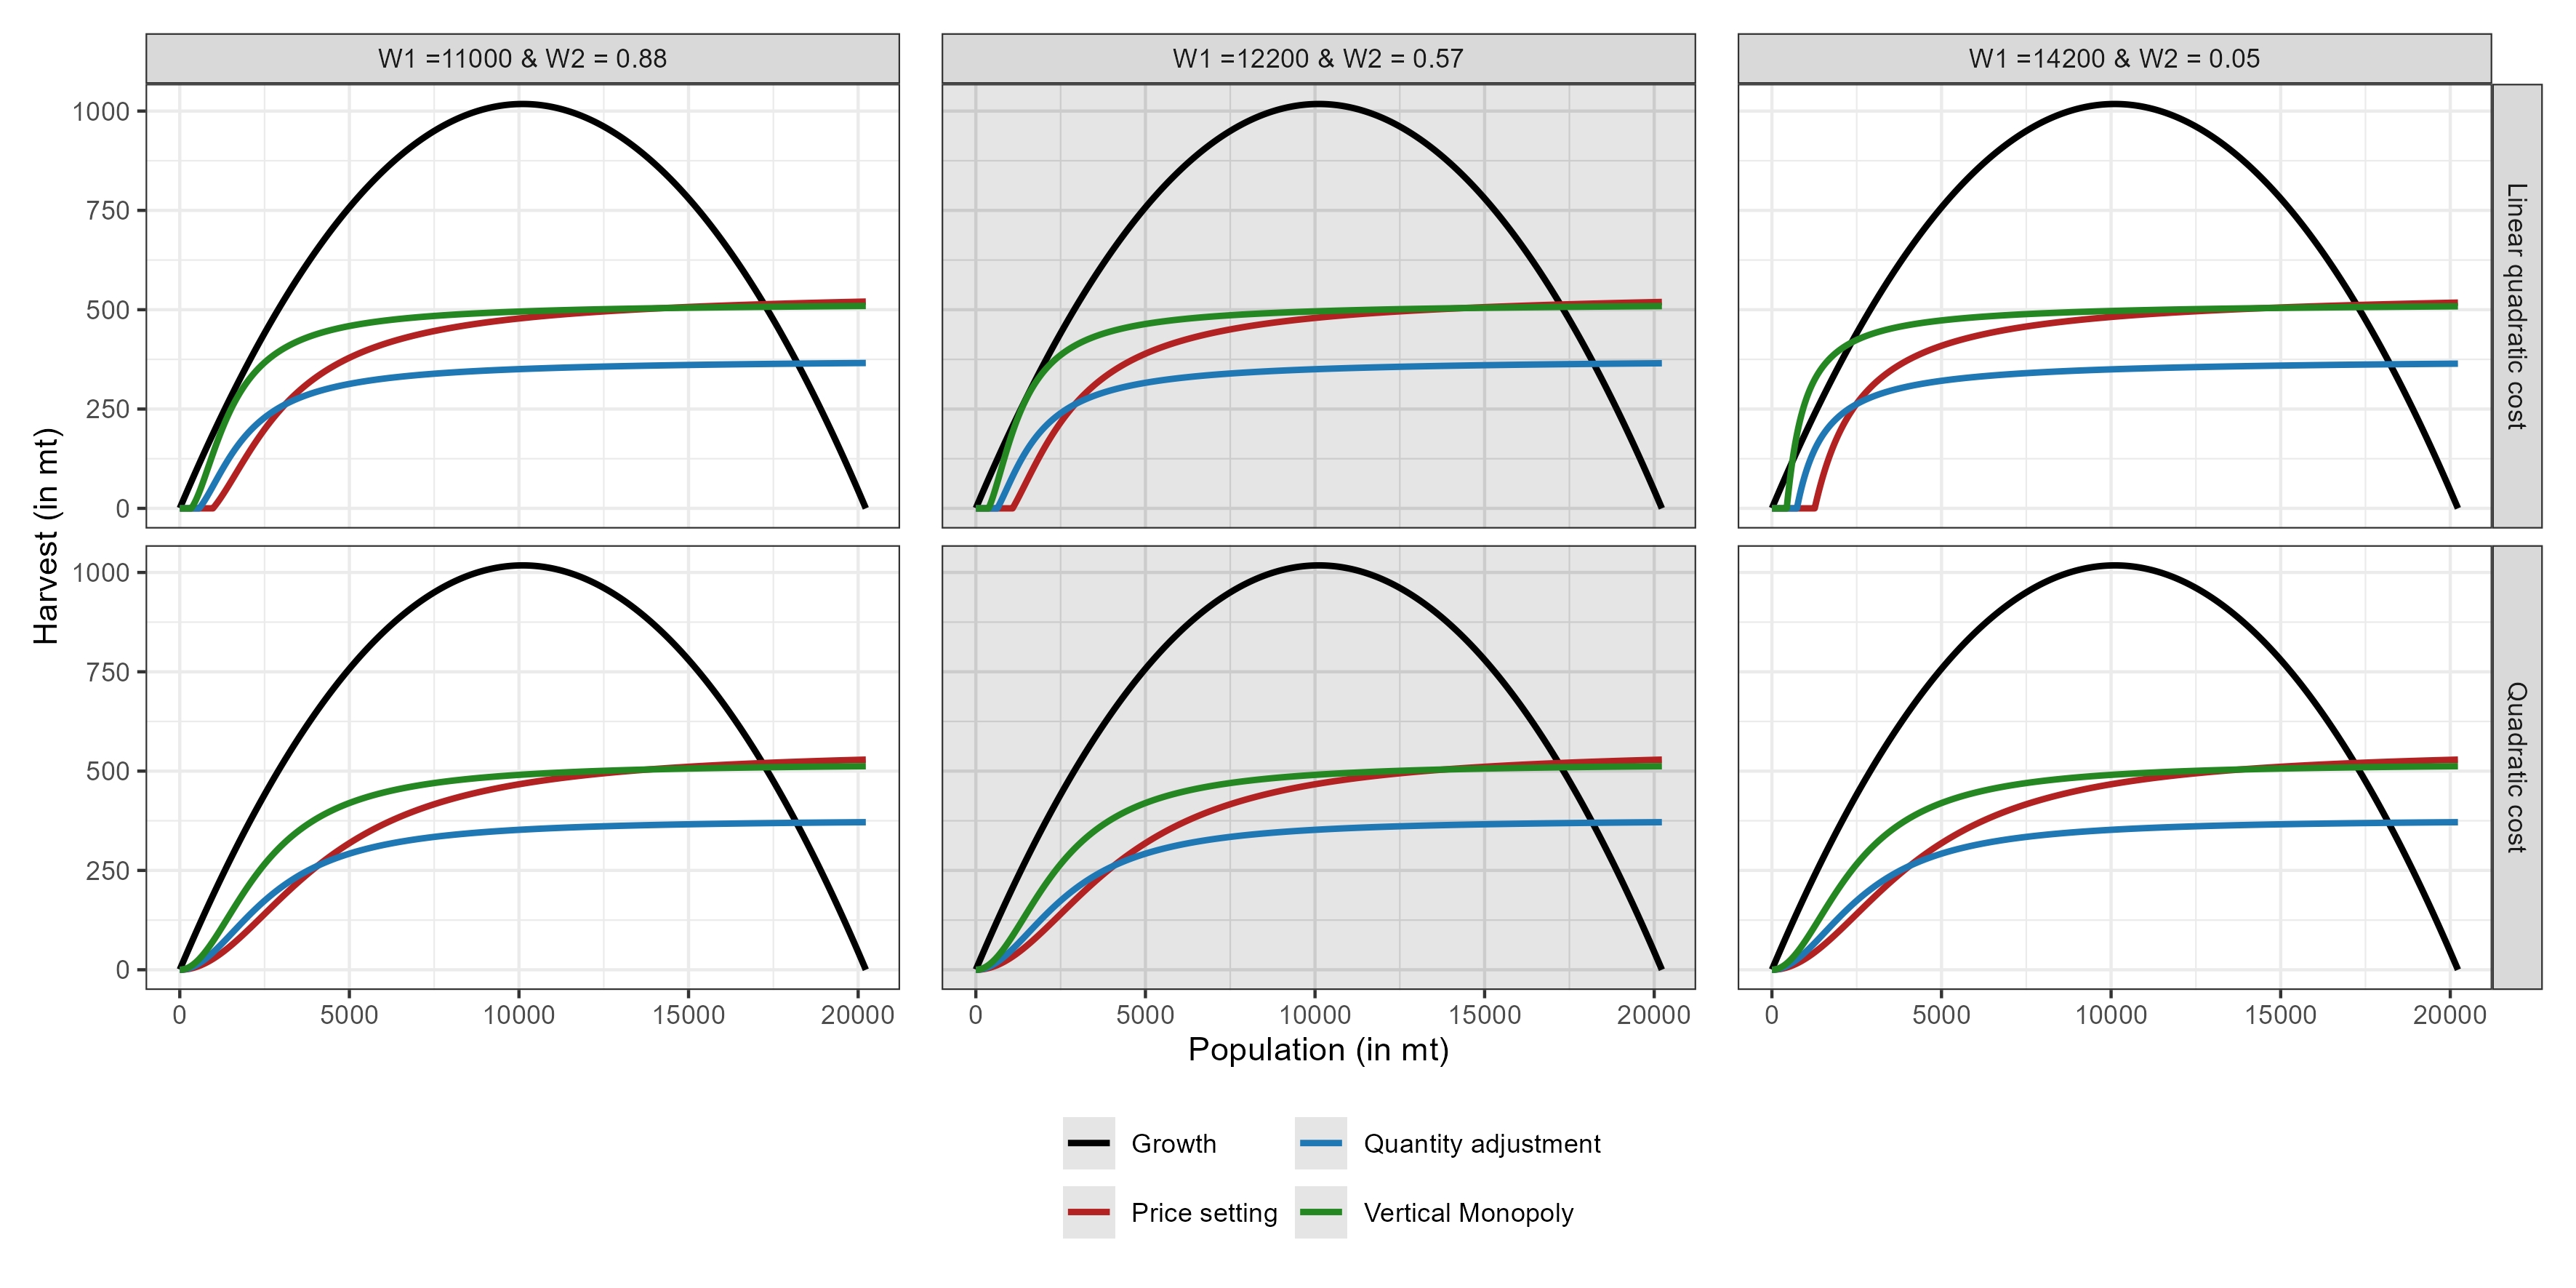
\includegraphics[width=0.85\linewidth]{figures/totoaba/figure4.png}
    \caption{ Sensitivity of equilibrium points to cost structure for wild totoaba stock}
    \subcaption*{Logistic growth function (black) for Totoaba macdonaldi wild stock biomass with intersecting colored lines representing different market structures and competitive responses. Harvest under the status quo vertical monopoly is represented by the green curve. When conservation farming is added to the monopoly scenario the trader can respond either in a mutually beneficial way by adjusting the quantity supplied given a market price (quantity adjustment, in blue). Alternatively, the trader can respond aggressively and try to set a price that undercuts the price of farmed products, resulting in increased poaching (price setting, in red). Cost parameters $W_1$ and $W_2$ correspond to the linear quadratic cost structure. In the top panel, equilibria are displayed for the linear quadratic cost, on the bottom, for a quadratic cost. On the left panel, the quadratic component is large, and vertical monopoly maintains a healthy stock. Center panel highlights the baseline scenario. In the right panel, the cost structure is close to linear. In this case, the vertical monopoly may lead to drastic stock decline.}
    \label{fig:figure5}
\end{figure}

\subsection{Farming produces conservation benefits}

While our results show that totoaba stock may remain healthy under the current monopolistic market conditions, these results are sensitive to changes in poaching costs (Figure \ref{fig:figure5}). Therefore, we ask if conservation farming can improve upon the status quo by producing a robust single high stable equilibrium point and reduced cartel profits.

We add conservation farming to the monopolist model and now have two ‘firms’ – a trader and a farmer – competing on a duopolistic market. When farming supplies legal product to end-market consumers, the demand for illegal product will fall, assuming that wild and farmed products are substitutable (an assumption we explore later). The monopolist trader can respond to competition in two ways: a mutually beneficial way by adjusting the quantity supplied given a market price (quantity adjustment), or alternatively, an aggressive way that tries to select a price that undercuts the price of farmed products (price setting). In both scenarios, the trader and farmer choose a quantity supplied simultaneously, without knowing how the other will respond. 
\\
Illegal markets are almost always characterized as competing through quantity adjustment \citep{poret_optimal_2009, flores_violence_2016}. Under the assumption that products are substitutable, it is more profitable – and therefore more likely – for both firms to compete through quantity adjustment \citep{singh_price_1984}. When goods are substitutes, if both firms restrict the quantities supplied, they both enjoy higher prices. If they flood the market, prices and profits collapse. In the case of totoaba, we find that if traders respond through quantity adjustment under the linear quadratic cost structure, then the wild stock biomass increases by $5.45\%$ (compared to a monopoly) to a steady state equilibrium of $18,220$ mt, or to $90\%$ of carrying capacity (Table \ref{fig:table}). This represents a reduction in poaching harvest of $28.27\%$ and $\$195.16$ million USD of annual lost profit to the trader.

Even if traders respond aggressively through price setting, considered a less likely response \citep{singh_price_1984} a single high equilibrium emerges (Figure \ref{fig:figure4}). Price setting is considered a much less likely response to competition because the trader would face steep profit losses. Under the high steady-state equilibrium with the linear quadratic cost structure, wild stock biomass decreases by $0.24\%$ relative to monopoly, to a steady-state equilibrium of $17,235$ mt, or to $85\%$ of carrying capacity (Table \ref{fig:table}). Although the high steady-state reflects a relatively small increase in poaching harvest by $5.85\%$, it would result in $\$313.84$ million USD of annual lost profit to the cartel, making this strategy unlikely. 

\begin{figure}[h]
    \centering
    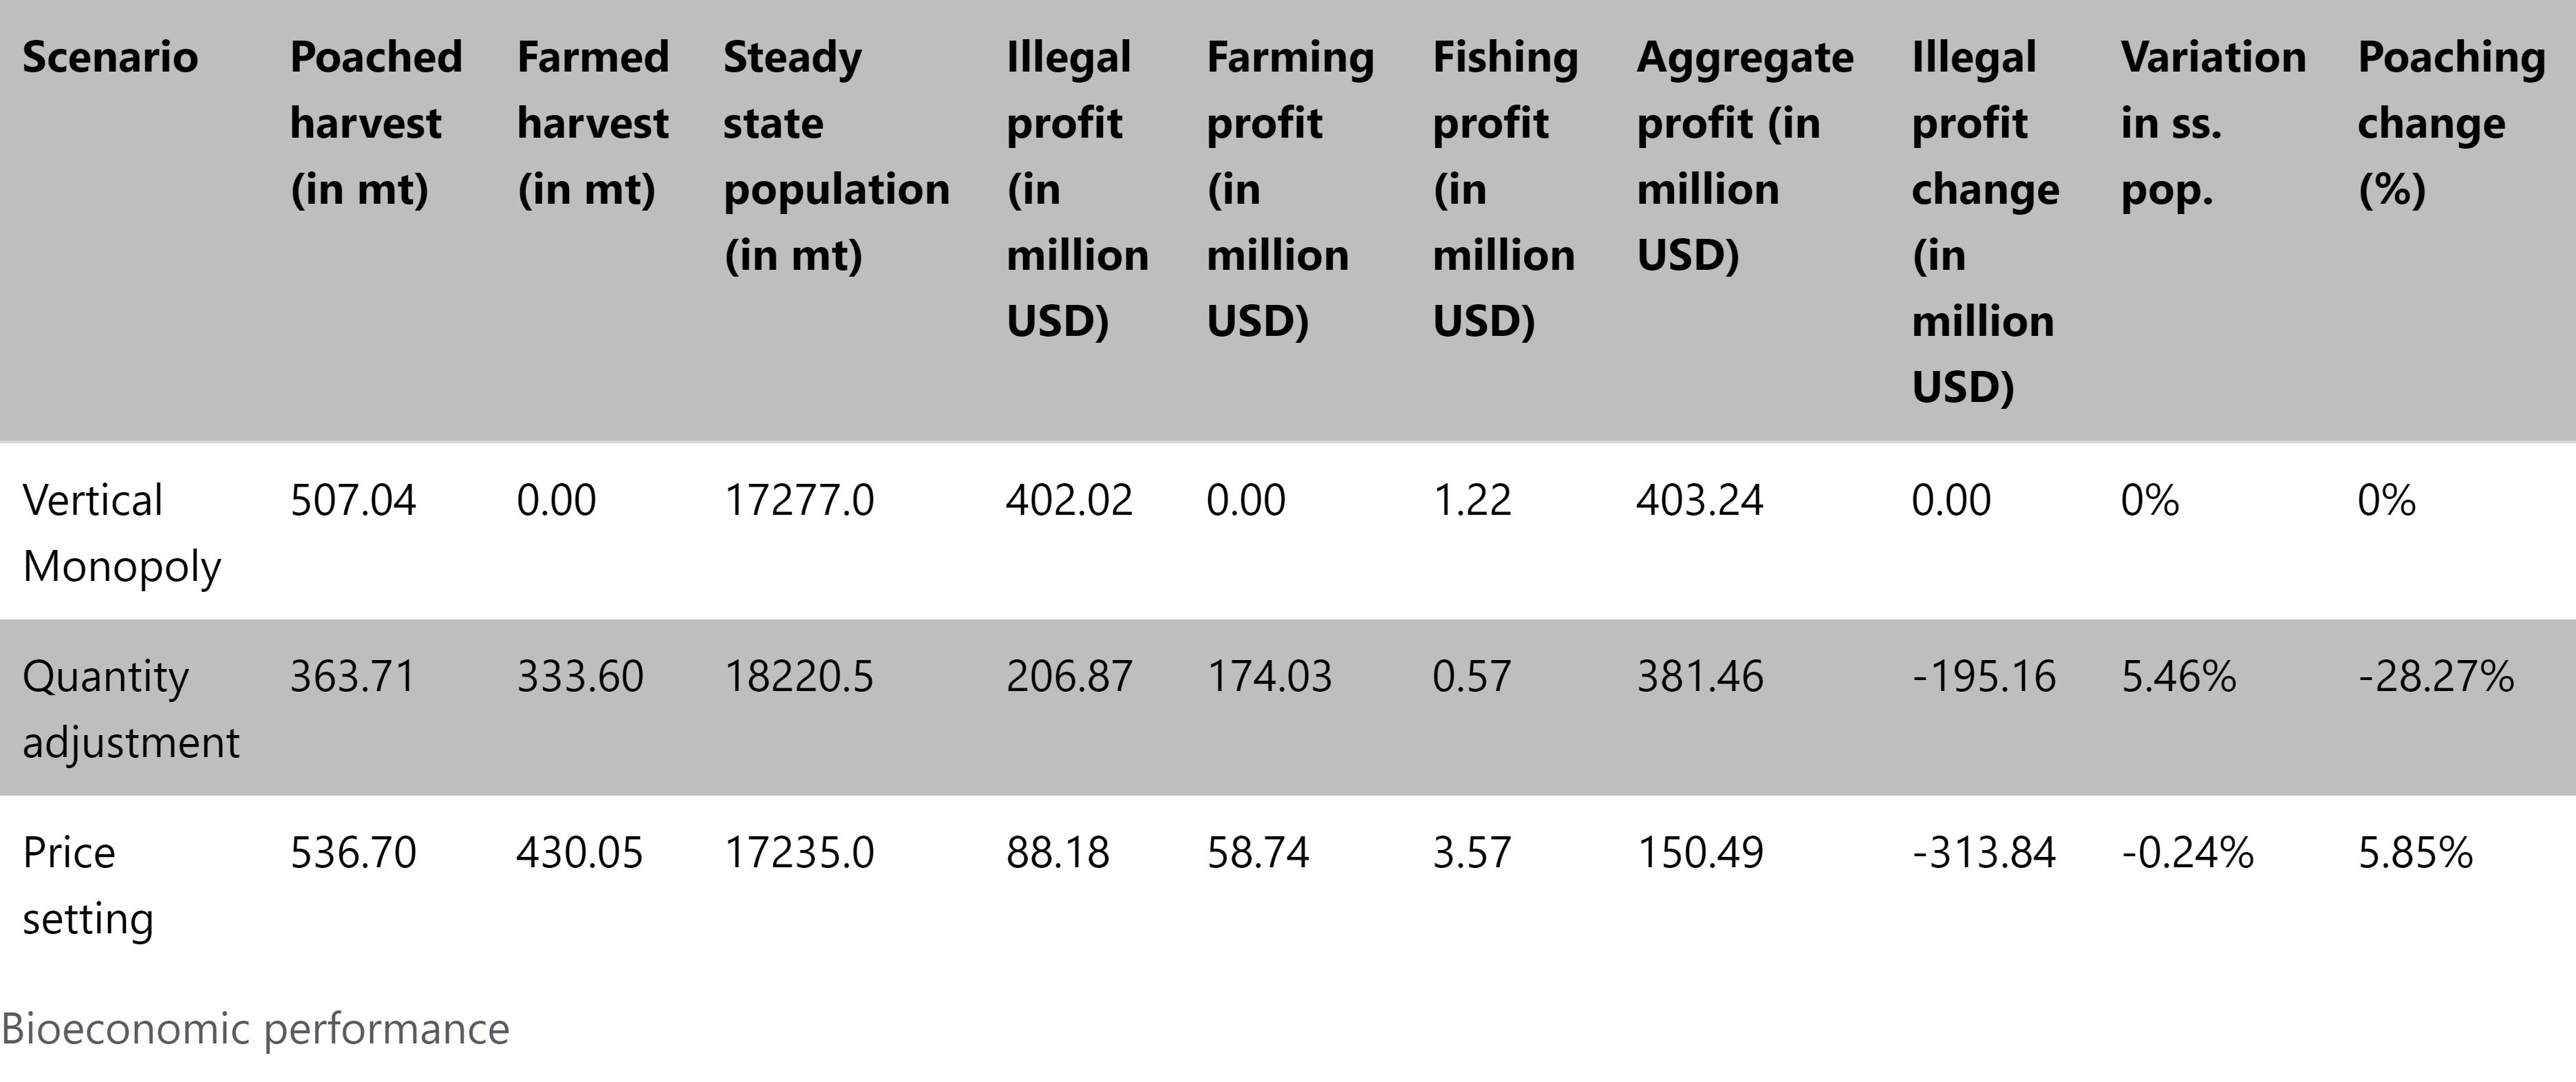
\includegraphics[width=0.85\linewidth]{figures/totoaba/bioecon_perf.png}
    \caption{Economic and ecological performance of different market regimes}
    \label{fig:table}
\end{figure}

Our current specifications for totoaba show that price setting leads to a slight increase in poaching pressure, however, we argue that price setting does not universally lead to increased poaching pressure, challenging a key conclusion from the original bioeconomic model \citep{bulte_economic_2005, damania_economics_2007}. Farming puts an upper bound on the price traders can pay to poachers in order to remain competitive. When the cost of farming becomes lower than the combined cost of poaching and trading, price-setting competition does not inevitably result in the overexploitation of the wild stock. This is because when farming costs are low, traders have an incentive to maintain large stocks by poaching less to remain competitive with farmers. This limits the price paid to poachers. On the other hand, when farming costs are large, traders have an incentive to poach more, paying a larger price to poachers while remaining competitive with the farming sector.  In the case of totoaba, species specific traits and market characteristics result in a slight increase in poaching in the price setting scenario. However, if the carrying capacity were smaller, or demand lower, the price-setting equilibrium would result in conservation benefits. 

While we focus on the effect of conservation farming on a monopolistic market structure, given that this scenario best represents the totoaba fishery today, the effect of conservation farming on market structures can be explored in different contexts. We model alternative market structures, including scenarios with multiple competing traders or multiple competing farmers, and find that if the number of farmers exceeds the number of traders, poaching levels will decline (supplementary figure \ref{fig:cournot_oligo}). Additionally, if farming is taken over by monopolists, we find that poaching is reduced and the wild population increases (supplementary figure \ref{fig:extended_cartel}).

\subsection{An effective policy space for farming.}

Our analysis provides a quantitative framework that can identify an effective policy space where all supply, demand, and market structure parameters align to ensure that conservation farming will reduce poaching, improving greatly on the original bioeconomic model and the limitations of binary qualitative approaches \citep{phelps_framework_2014,tensen_under_2016, bulte_economic_2005, damania_economics_2007, challender_evaluating_2019}. This bioeconomic model allows researchers to quantify: (a) how much cheaper farming must be relative to poaching to be competitive; (b) how much of a demand increase can be absorbed by farming; and (c) how substitutable must wildlife products be for farmed products to displace wild products. Critically, we also explore how the interaction between these factors may affect outcomes. We explore how sensitive the results are for totoaba, offering general and totoaba-specific policy solutions to help ensure that conservation farming remains in the effective policy space.

We find that the cost of conservation farming for totoaba can be high and still competitive with poaching, but this is contingent on the cost for traders also being high (supplementary figure \ref{fig:c_and_v}). Traders inherently rely on poachers to obtain totoaba, and if farming is expensive this forces traders to pay poachers higher prices. If traders compete with poachers under the more likely quantity adjustment response, the population remains healthy, even increasing by nearly $6\%$ from the monopoly steady state. However, if traders compete with farmers by price setting, the low prices paid to poachers can incentivize poachers to increase fishing pressure in order to maintain payouts. This can lead to a decrease in the wild population biomass modestly by $0.24\%$ from the monopoly steady state. Policymakers can support farming success by subsidizing farming to keep the cost low while maintaining enforcement to keep the cost of poaching high (for totoaba this includes marine patrols, fisheries closures, and gillnet bans). To mitigate the possibility of stock decline under the less-likely price-setting response, we identify that maintaining conservation farming below $\$77,339$ USD per mt of totoaba (amounting to a $14\%$ subsidy on unit production cost) will prevent any increase in poaching pressure under either competitive response, assuming no effect of law enforcement in our baseline model.


\begin{figure}[h]
    \centering
    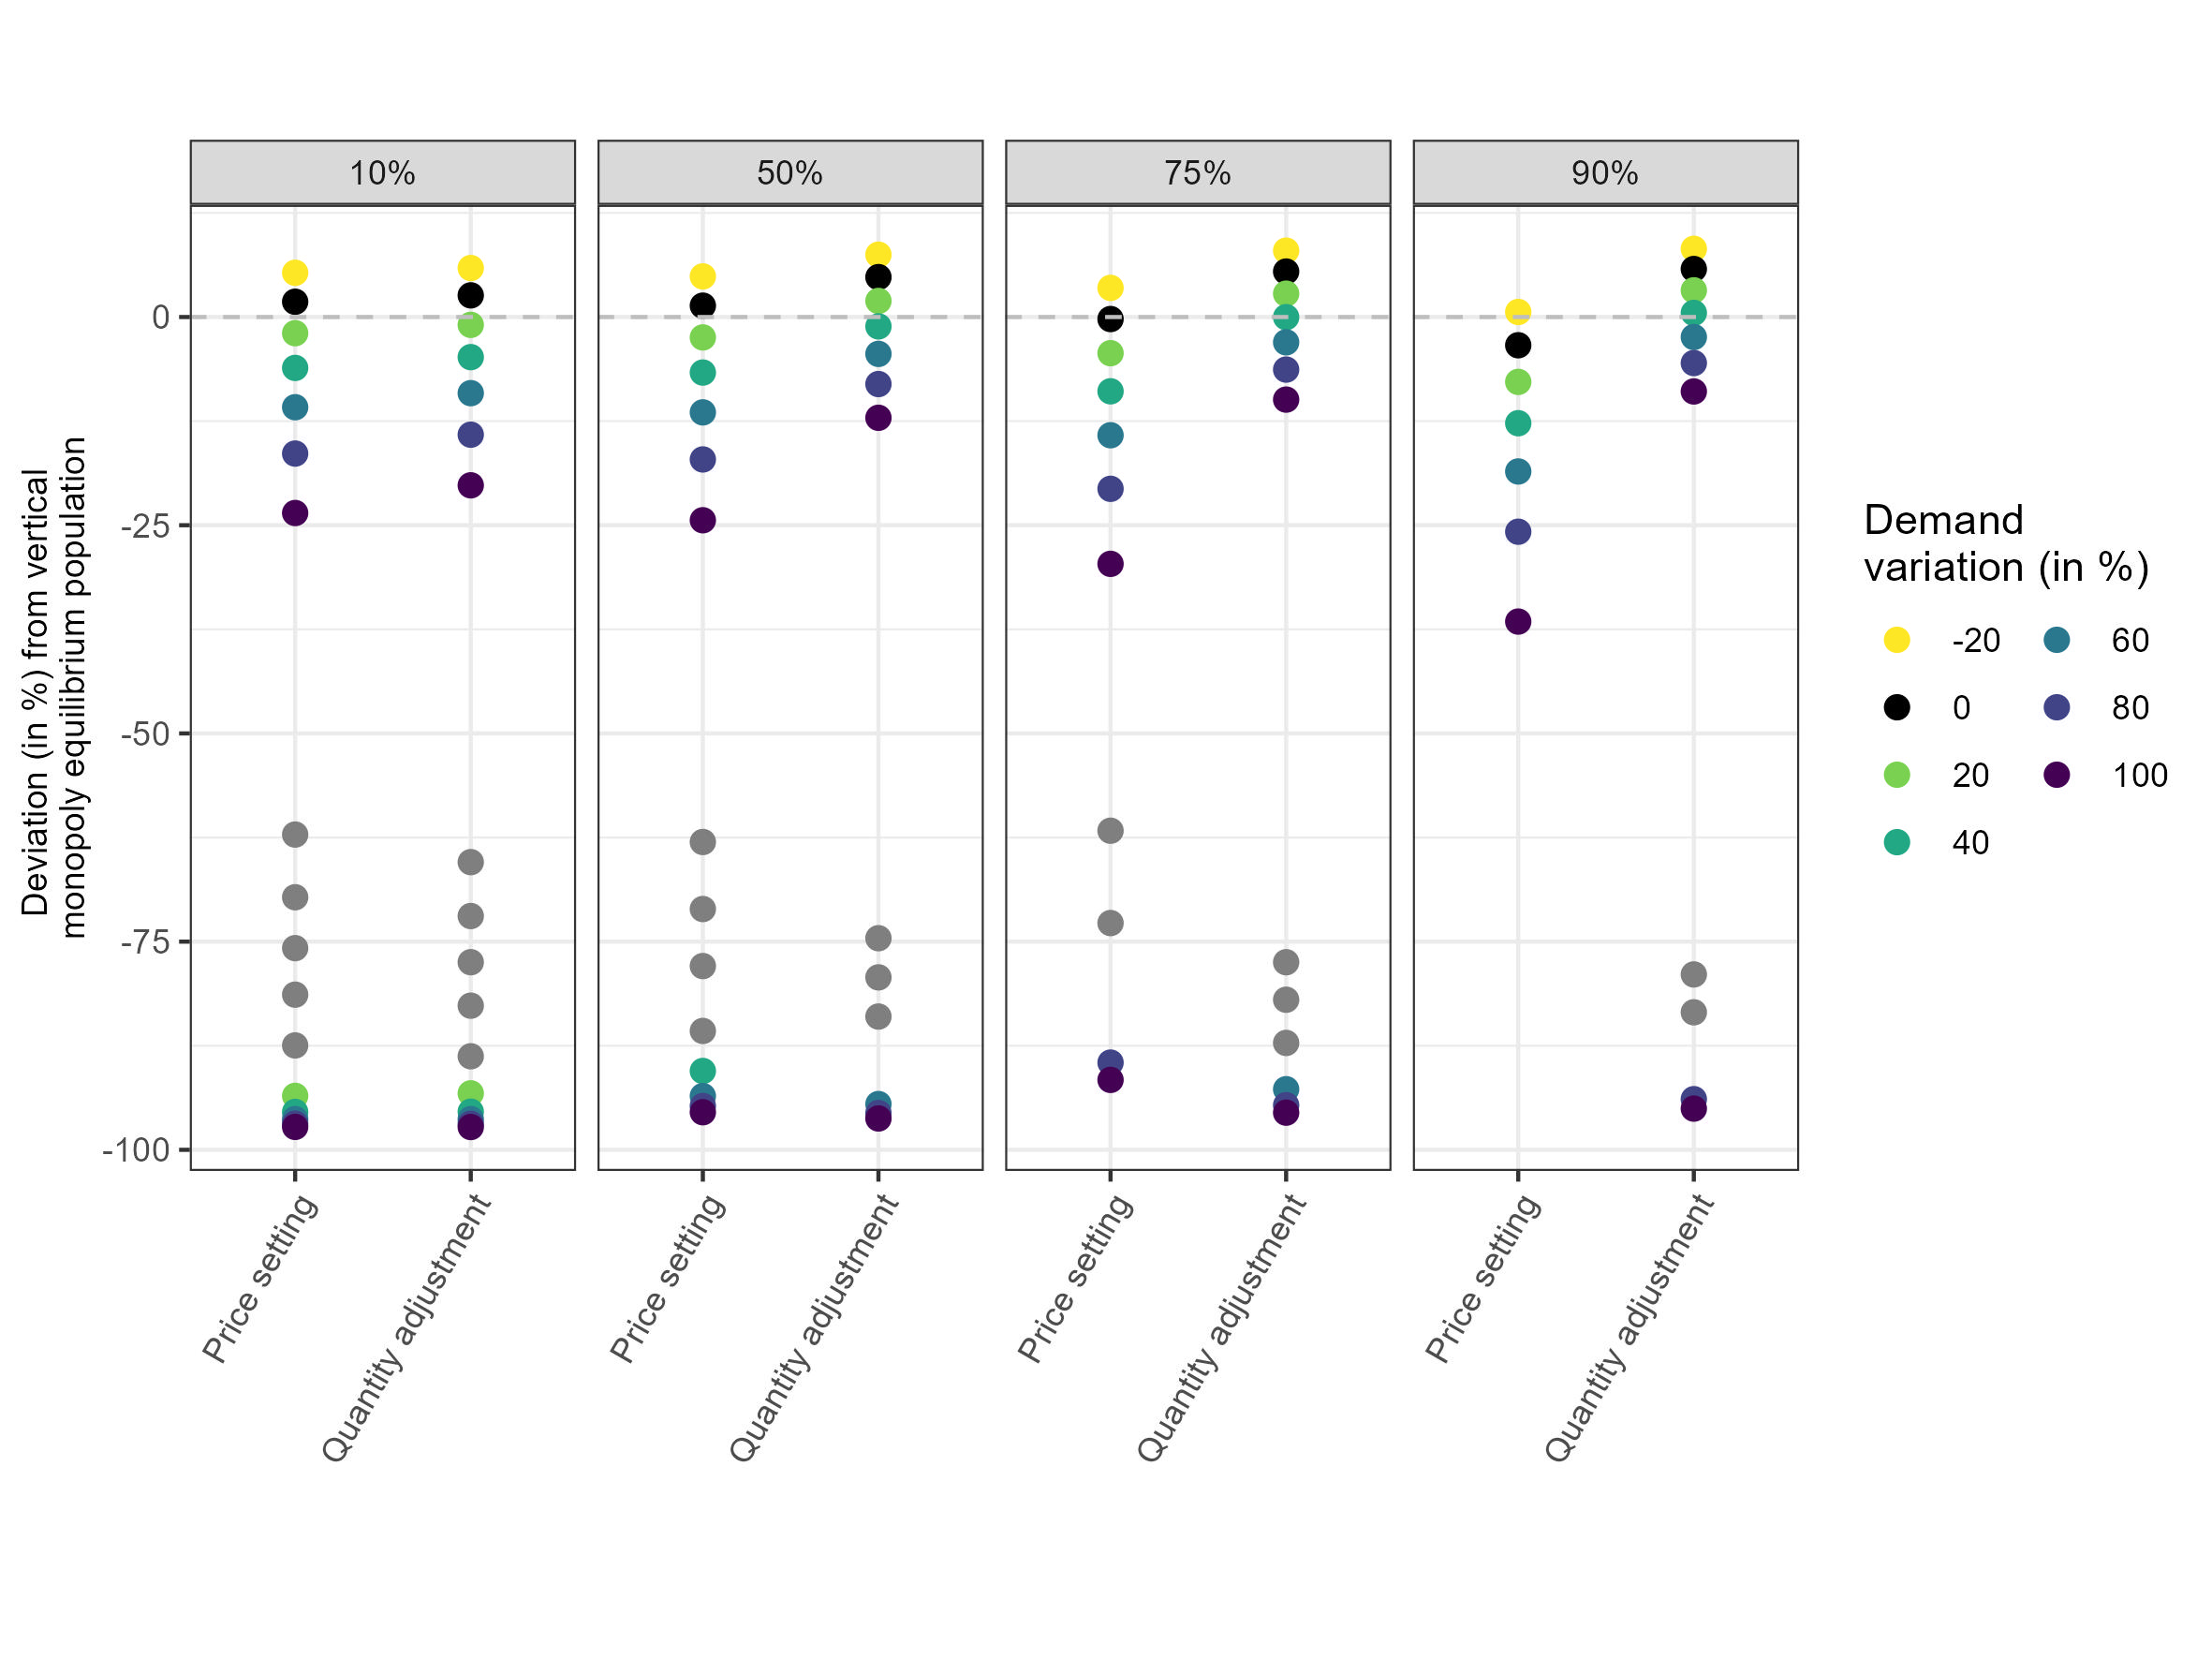
\includegraphics[width=0.85\linewidth]{figures/totoaba/Figure5.jpg}
    \caption{Interaction between substitutability and demand under duopolistic competition}
    \subcaption*{Each panel represents a different substitutability between farmed and wild product: large ($90\%$ substitutability), baseline ($75\%$), medium ($50\%$ substitutability), and low (10\% substitutability). Our baseline results are in the $75\%$ substitutability case, with zero demand variation (black dots) When conservation farming is added to the monopoly scenario the trader can respond aggressively and try to set a price that undercuts the price of farmed products (price setting), alternatively the trader can respond in a mutually beneficial way by adjusting the quantity supplied given a market price (quantity adjustment). We simulate a change in end-market demand ranging from a reduction in demand by $20\%$ to an increase in demand up to $100\%$, in increments of $20\%$. One, two, or three potential equilibria can emerge. Where three equilibrium points emerge, we color only the high and low stable equilibria (unstable equilibria are indicated in gray). The dotted horizontal lines indicate the status quo monopoly equilibrium population (in the absence of conservation farming). Points closer to 0 represent a high stable equilibrium point, whereas points closer to $-100$ represent a population collapse stable equilibrium point.}
    \label{fig:figure6}
\end{figure}

Our results confirm that high substitutability is critical to conservation farming success and leads to larger conservation benefits in the quantity-setting equilibrium, under the assumption that demand remains stable (Figure \ref{fig:figure6}). Fish swim bladders have a wide variety of uses and values, and it is possible that farmed totoaba swim bladders may enter into these different product streams \citep{sadovy_de_mitcheson_emerging_2019}. In the case of no substitutability, two separate, non-competitive markets emerge. In this scenario the status quo is maintained, both firms set high prices, and traders continue to operate as a monopoly because farmed product does not compete with wild product. At the other extreme, in the case of perfect substitutability, consumers prefer the cheaper option without any preference of source. This increases the intensity of potential price-setting competition between firms and further depletes the stock in this case. To comply with CITES captive breeding guidelines totoaba must be identified as farmed \citep{cites_additional_2019}, and distinguishing between products to meet regulatory obligations can artificially lower substitutability. Outcomes vary under intermediate states of substitutability. For low to medium substitutability (i.e., $10-50\%$) traders and farmers are still likely to limit quantity: undercutting a competitor would yield significant profit losses. For high substitutability (i.e., $90\%$) there is an incentive to compete for market control either by price setting or quantity adjustment, which reflects our main results. 

The value of totoaba swim bladder is tied to rarity, and while demand evolution is an open empirical question, we test the sensitivity of our results to simultaneous changes in demand and substitutability (Figure \ref{fig:figure6}). Totoaba swim bladder purchases are ‘conspicuous consumption,’ luxury products commonly purchased for social status and speculative investing by wealthy consumers \citep{sadovy_de_mitcheson_emerging_2019, veblen_theory_2023}. A decrease in swim bladder price resulting from conservation farming may actually undermine the desirability of totoaba swim bladders in Chinese end markets, given that the high monetary value is linked to high social status \citep{jinkins_conspicuous_2016}. However, some increase in demand may be expected if a legal product becomes available, as law-abiding consumers will be more likely to purchase wildlife products when those products are traded and purchased legally \citep{phelps_framework_2014}. Under our high substitutability assumption ($75\%$), competition through quantity adjustment can withstand a $40\%$ increase in demand, whereas competition through price setting is not robust to demand increases. For price setting, a demand increase of $40\%$ would cause the equilibrium population to decrease by $10\%$ from the monopoly status quo, increasing poaching by $216$ mt. 

There is a much higher threat to the wild population if demand increases under low to medium substitutability (i.e. $10-50\%$), given that this additional demand cannot be fully met by farmed product (Figure \ref{fig:figure6}). In the best-case and most likely scenario, medium substitutability ($50\%$) can meet a $20\%$ increase in demand if competition occurs through quantity adjustment, although uncertain outcomes (e.g. high and low steady states) start to emerge if demand increases by $60\%$ or more. In the worst-case scenario, if competition occurs through price setting and products have medium substitutability ($50\%$), any increase in demand reduces the wild population from the status quo. While increases in demand of $20-40\%$ still produce a single high equilibrium point, the population size is lower than under monopoly. Furthermore, if demand increases beyond $80\%$, uncertain outcomes emerge, with the wild population either stabilizing at a high equilibrium point ($14,322$ mt in the price setting scenario; $15,886$ mt in the quantity adjustment scenario) or being pushed to a low equilibrium point (ranging from $763$ mt in the quantity adjustment scenario; $909$ mt in the price setting scenario). We recommend that stated preference investigations on wild versus farmed product should be undertaken in Chinese end-markets and that these investigations include questions focused on perceived social status benefit and legality \citep{hinsley_wild_2020}. 

\section{Conclusion}
Our results show that conservation farming presents a potentially high reward intervention. If traders respond to competition from farming by quantity adjustment, the wild totoaba stock is predicted to increase by $5.45\%$ relative to the status quo monopoly, to a high stable biomass of $18,220$ mt ($90\%$ of carrying capacity). In addition to improving the totoaba wild stock, this quantity adjustment response will decrease poaching by $28.27\%$ relative to the status quo. If traders respond by price setting, the wild stock biomass decreases by less than $1\%$ to a high stable biomass of $17,235$ mt ($85\%$ of carrying capacity). Economic theory concludes that quantity adjustment is the more likely outcome because restricting quantities allows both farmers and traders to collect higher profits \citep{singh_price_1984}. Conservation farming presents a more robust outcome to the status quo monopoly market structure (where a single trader dominates the market), as the wild totoaba reaches either a low or high stable equilibrium biomass depending on the poaching cost structure. We find that if products have high substitutability they are more likely to maintain a high stable equilibrium. Further, under a quantity adjustment response, highly substitutable products can better maintain this high stable equilibrium for demand increases up to $40\%$. Our results are sensitive to changes in substitutability and increases in demand, therefore we encourage a thorough understanding of end-market demand before implementing conservation farming for totoaba.

We revive an existing bioeconomic model and reach different and optimistic conclusions about the potential for conservation farming to reduce poaching and maintain a healthy wild population. We provide a novel framework to objectively assess the potential effects of farming by grounding our analysis in detailed species ecology and market data. Furthermore, our approach provides a rigorous alternative to existing qualitative frameworks that are unable to analyze the interaction between multiple variables. While our analysis focuses on totoaba, the bioeconomic model is flexible and can be applied more broadly to other species and contexts to examine the effect of conservation farming on a wild population. 


%\section{Methods}

\subsubsection*{Acknowledgements}
We thank Mark Buntaine, Chris Costello, and Lauriane Mouysset for helpful comments and feedback on the manuscript, as well as members of the Costello research group. J.M.L acknowledges funding from the Daniel and Dianne Vapnek Fisheries Management Fellowship, the Schmidt Family Foundation Research Accelerator Award as well as from the National Sciences and Engineering Research Council of Canada (NSERC) Postgraduate Scholarship. M.C.-R. acknowledges funding from the Latin American Fisheries Fellowship. 

\section*{Contributions and data availability}

J.M.L and S.J contributed to this work equally. J.M.L., S.J., M.C-R., G.M.G., M.A.C-M., E.A-B, and S.D.G. contributed to writing the manuscript. J.M.L., S.J., A.S., and S.D.G. contributed to study conception and design. All authors contributed to data acquisition and analysis. All authors approve of the submitted manuscript.
\\
The data that support the findings of this study are available  \href{https://doi.org/10.17605/OSF.IO/6Y8CQ}{here}
\\
The code used for this study is publicly available on \href{https://github.com/julawson/conservation_farming_totoaba}{Github} and \href{https://doi.org/10.17605/OSF.IO/6Y8CQ}{archived here}

